% GNUPLOT: LaTeX picture with Postscript
\begingroup
  \makeatletter
  \providecommand\color[2][]{%
    \GenericError{(gnuplot) \space\space\space\@spaces}{%
      Package color not loaded in conjunction with
      terminal option `colourtext'%
    }{See the gnuplot documentation for explanation.%
    }{Either use 'blacktext' in gnuplot or load the package
      color.sty in LaTeX.}%
    \renewcommand\color[2][]{}%
  }%
  \providecommand\includegraphics[2][]{%
    \GenericError{(gnuplot) \space\space\space\@spaces}{%
      Package graphicx or graphics not loaded%
    }{See the gnuplot documentation for explanation.%
    }{The gnuplot epslatex terminal needs graphicx.sty or graphics.sty.}%
    \renewcommand\includegraphics[2][]{}%
  }%
  \providecommand\rotatebox[2]{#2}%
  \@ifundefined{ifGPcolor}{%
    \newif\ifGPcolor
    \GPcolortrue
  }{}%
  \@ifundefined{ifGPblacktext}{%
    \newif\ifGPblacktext
    \GPblacktexttrue
  }{}%
  % define a \g@addto@macro without @ in the name:
  \let\gplgaddtomacro\g@addto@macro
  % define empty templates for all commands taking text:
  \gdef\gplbacktext{}%
  \gdef\gplfronttext{}%
  \makeatother
  \ifGPblacktext
    % no textcolor at all
    \def\colorrgb#1{}%
    \def\colorgray#1{}%
  \else
    % gray or color?
    \ifGPcolor
      \def\colorrgb#1{\color[rgb]{#1}}%
      \def\colorgray#1{\color[gray]{#1}}%
      \expandafter\def\csname LTw\endcsname{\color{white}}%
      \expandafter\def\csname LTb\endcsname{\color{black}}%
      \expandafter\def\csname LTa\endcsname{\color{black}}%
      \expandafter\def\csname LT0\endcsname{\color[rgb]{1,0,0}}%
      \expandafter\def\csname LT1\endcsname{\color[rgb]{0,1,0}}%
      \expandafter\def\csname LT2\endcsname{\color[rgb]{0,0,1}}%
      \expandafter\def\csname LT3\endcsname{\color[rgb]{1,0,1}}%
      \expandafter\def\csname LT4\endcsname{\color[rgb]{0,1,1}}%
      \expandafter\def\csname LT5\endcsname{\color[rgb]{1,1,0}}%
      \expandafter\def\csname LT6\endcsname{\color[rgb]{0,0,0}}%
      \expandafter\def\csname LT7\endcsname{\color[rgb]{1,0.3,0}}%
      \expandafter\def\csname LT8\endcsname{\color[rgb]{0.5,0.5,0.5}}%
    \else
      % gray
      \def\colorrgb#1{\color{black}}%
      \def\colorgray#1{\color[gray]{#1}}%
      \expandafter\def\csname LTw\endcsname{\color{white}}%
      \expandafter\def\csname LTb\endcsname{\color{black}}%
      \expandafter\def\csname LTa\endcsname{\color{black}}%
      \expandafter\def\csname LT0\endcsname{\color{black}}%
      \expandafter\def\csname LT1\endcsname{\color{black}}%
      \expandafter\def\csname LT2\endcsname{\color{black}}%
      \expandafter\def\csname LT3\endcsname{\color{black}}%
      \expandafter\def\csname LT4\endcsname{\color{black}}%
      \expandafter\def\csname LT5\endcsname{\color{black}}%
      \expandafter\def\csname LT6\endcsname{\color{black}}%
      \expandafter\def\csname LT7\endcsname{\color{black}}%
      \expandafter\def\csname LT8\endcsname{\color{black}}%
    \fi
  \fi
    \setlength{\unitlength}{0.0500bp}%
    \ifx\gptboxheight\undefined%
      \newlength{\gptboxheight}%
      \newlength{\gptboxwidth}%
      \newsavebox{\gptboxtext}%
    \fi%
    \setlength{\fboxrule}{0.5pt}%
    \setlength{\fboxsep}{1pt}%
    \definecolor{tbcol}{rgb}{1,1,1}%
\begin{picture}(7480.00,4320.00)%
    \gplgaddtomacro\gplbacktext{%
      \csname LTb\endcsname%%
      \put(645,2773){\makebox(0,0)[r]{\strut{}0}}%
      \csname LTb\endcsname%%
      \put(645,3020){\makebox(0,0)[r]{\strut{}10}}%
      \csname LTb\endcsname%%
      \put(645,3268){\makebox(0,0)[r]{\strut{}20}}%
      \csname LTb\endcsname%%
      \put(645,3515){\makebox(0,0)[r]{\strut{}30}}%
      \csname LTb\endcsname%%
      \put(645,3762){\makebox(0,0)[r]{\strut{}40}}%
      \csname LTb\endcsname%%
      \put(645,4009){\makebox(0,0)[r]{\strut{}50}}%
      \csname LTb\endcsname%%
      \put(645,4256){\makebox(0,0)[r]{\strut{}60}}%
      \csname LTb\endcsname%%
      \put(746,2533){\makebox(0,0){\strut{}0.00}}%
      \csname LTb\endcsname%%
      \put(1138,2533){\makebox(0,0){\strut{}0.01}}%
      \csname LTb\endcsname%%
      \put(1531,2533){\makebox(0,0){\strut{}0.02}}%
      \csname LTb\endcsname%%
      \put(1924,2533){\makebox(0,0){\strut{}0.03}}%
      \csname LTb\endcsname%%
      \put(2317,2533){\makebox(0,0){\strut{}0.04}}%
      \csname LTb\endcsname%%
      \put(2710,2533){\makebox(0,0){\strut{}0.05}}%
    }%
    \gplgaddtomacro\gplfronttext{%
      \csname LTb\endcsname%%
      \put(248,3515){\rotatebox{-270.00}{\makebox(0,0){\strut{}kf [MPa]}}}%
    }%
    \gplgaddtomacro\gplbacktext{%
      \csname LTb\endcsname%%
      \put(2982,2773){\makebox(0,0)[r]{\strut{}}}%
      \csname LTb\endcsname%%
      \put(2982,3020){\makebox(0,0)[r]{\strut{}}}%
      \csname LTb\endcsname%%
      \put(2982,3268){\makebox(0,0)[r]{\strut{}}}%
      \csname LTb\endcsname%%
      \put(2982,3515){\makebox(0,0)[r]{\strut{}}}%
      \csname LTb\endcsname%%
      \put(2982,3762){\makebox(0,0)[r]{\strut{}}}%
      \csname LTb\endcsname%%
      \put(2982,4009){\makebox(0,0)[r]{\strut{}}}%
      \csname LTb\endcsname%%
      \put(2982,4256){\makebox(0,0)[r]{\strut{}}}%
      \csname LTb\endcsname%%
      \put(3083,2533){\makebox(0,0){\strut{}0.00}}%
      \csname LTb\endcsname%%
      \put(3476,2533){\makebox(0,0){\strut{}0.02}}%
      \csname LTb\endcsname%%
      \put(3869,2533){\makebox(0,0){\strut{}0.04}}%
      \csname LTb\endcsname%%
      \put(4262,2533){\makebox(0,0){\strut{}0.06}}%
      \csname LTb\endcsname%%
      \put(4654,2533){\makebox(0,0){\strut{}0.08}}%
      \csname LTb\endcsname%%
      \put(5047,2533){\makebox(0,0){\strut{}0.10}}%
    }%
    \gplgaddtomacro\gplfronttext{%
    }%
    \gplgaddtomacro\gplbacktext{%
      \csname LTb\endcsname%%
      \put(645,860){\makebox(0,0)[r]{\strut{}0}}%
      \csname LTb\endcsname%%
      \put(645,1156){\makebox(0,0)[r]{\strut{}20}}%
      \csname LTb\endcsname%%
      \put(645,1453){\makebox(0,0)[r]{\strut{}40}}%
      \csname LTb\endcsname%%
      \put(645,1750){\makebox(0,0)[r]{\strut{}60}}%
      \csname LTb\endcsname%%
      \put(645,2046){\makebox(0,0)[r]{\strut{}80}}%
      \csname LTb\endcsname%%
      \put(645,2343){\makebox(0,0)[r]{\strut{}100}}%
      \csname LTb\endcsname%%
      \put(746,620){\makebox(0,0){\strut{}0.0}}%
      \csname LTb\endcsname%%
      \put(1237,620){\makebox(0,0){\strut{}0.1}}%
      \csname LTb\endcsname%%
      \put(1728,620){\makebox(0,0){\strut{}0.1}}%
      \csname LTb\endcsname%%
      \put(2219,620){\makebox(0,0){\strut{}0.2}}%
      \csname LTb\endcsname%%
      \put(2710,620){\makebox(0,0){\strut{}0.2}}%
    }%
    \gplgaddtomacro\gplfronttext{%
      \csname LTb\endcsname%%
      \put(147,1601){\rotatebox{-270.00}{\makebox(0,0){\strut{}kf [MPa]}}}%
      \csname LTb\endcsname%%
      \put(1728,260){\makebox(0,0){\strut{}\varphi}}%
    }%
    \gplgaddtomacro\gplbacktext{%
      \csname LTb\endcsname%%
      \put(2982,860){\makebox(0,0)[r]{\strut{}}}%
      \csname LTb\endcsname%%
      \put(2982,1156){\makebox(0,0)[r]{\strut{}}}%
      \csname LTb\endcsname%%
      \put(2982,1453){\makebox(0,0)[r]{\strut{}}}%
      \csname LTb\endcsname%%
      \put(2982,1750){\makebox(0,0)[r]{\strut{}}}%
      \csname LTb\endcsname%%
      \put(2982,2046){\makebox(0,0)[r]{\strut{}}}%
      \csname LTb\endcsname%%
      \put(2982,2343){\makebox(0,0)[r]{\strut{}}}%
      \csname LTb\endcsname%%
      \put(3083,620){\makebox(0,0){\strut{}0.0}}%
      \csname LTb\endcsname%%
      \put(3410,620){\makebox(0,0){\strut{}0.1}}%
      \csname LTb\endcsname%%
      \put(3738,620){\makebox(0,0){\strut{}0.1}}%
      \csname LTb\endcsname%%
      \put(4065,620){\makebox(0,0){\strut{}0.2}}%
      \csname LTb\endcsname%%
      \put(4393,620){\makebox(0,0){\strut{}0.2}}%
      \csname LTb\endcsname%%
      \put(4720,620){\makebox(0,0){\strut{}0.2}}%
      \csname LTb\endcsname%%
      \put(5047,620){\makebox(0,0){\strut{}0.3}}%
    }%
    \gplgaddtomacro\gplfronttext{%
      \csname LTb\endcsname%%
      \put(4065,260){\makebox(0,0){\strut{}\varphi}}%
    }%
    \gplgaddtomacro\gplbacktext{%
      \csname LTb\endcsname%%
      \put(5320,860){\makebox(0,0)[r]{\strut{}}}%
      \csname LTb\endcsname%%
      \put(5320,1156){\makebox(0,0)[r]{\strut{}}}%
      \csname LTb\endcsname%%
      \put(5320,1453){\makebox(0,0)[r]{\strut{}}}%
      \csname LTb\endcsname%%
      \put(5320,1750){\makebox(0,0)[r]{\strut{}}}%
      \csname LTb\endcsname%%
      \put(5320,2046){\makebox(0,0)[r]{\strut{}}}%
      \csname LTb\endcsname%%
      \put(5320,2343){\makebox(0,0)[r]{\strut{}}}%
      \csname LTb\endcsname%%
      \put(5420,620){\makebox(0,0){\strut{}0.0}}%
      \csname LTb\endcsname%%
      \put(5748,620){\makebox(0,0){\strut{}0.1}}%
      \csname LTb\endcsname%%
      \put(6075,620){\makebox(0,0){\strut{}0.1}}%
      \csname LTb\endcsname%%
      \put(6403,620){\makebox(0,0){\strut{}0.2}}%
      \csname LTb\endcsname%%
      \put(6730,620){\makebox(0,0){\strut{}0.2}}%
      \csname LTb\endcsname%%
      \put(7057,620){\makebox(0,0){\strut{}0.2}}%
      \csname LTb\endcsname%%
      \put(7385,620){\makebox(0,0){\strut{}0.3}}%
    }%
    \gplgaddtomacro\gplfronttext{%
      \csname LTb\endcsname%%
      \put(6584,1315){\makebox(0,0)[r]{\strut{}data}}%
      \csname LTb\endcsname%%
      \put(6584,1075){\makebox(0,0)[r]{\strut{}f(x)}}%
      \csname LTb\endcsname%%
      \put(6403,260){\makebox(0,0){\strut{}\varphi}}%
    }%
    \gplbacktext
    \put(0,0){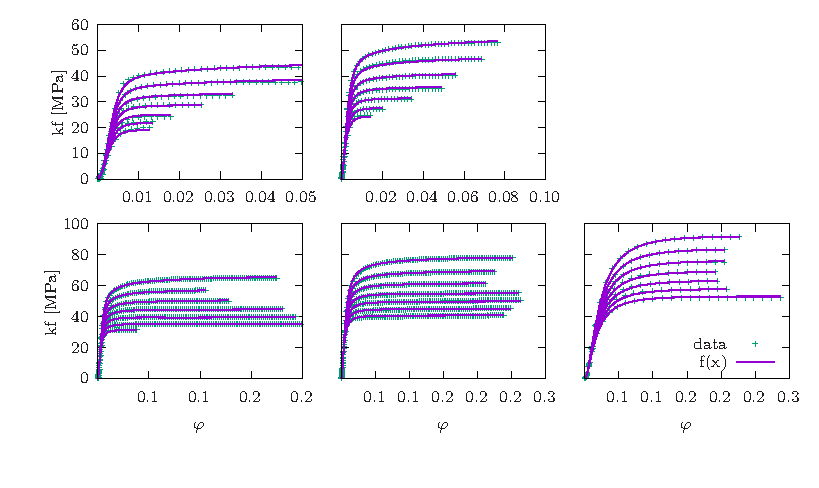
\includegraphics[width={374.00bp},height={216.00bp}]{linechart-alu-tomax-2row}}%
    \gplfronttext
  \end{picture}%
\endgroup
